\documentclass[11pt, letterpaper]{memoir}
\usepackage{HomeworkStyle}
\geometry{margin=1in}



\begin{document}

	\begin{center}
		{\large Quiz 5.3 -- Mixtures and Phases}
	\end{center}
	{\large Name: \rule[-1mm]{4in}{.1pt} 
		
\noindent 
Use the table below to estimate the vapor phase mole fraction ($y$) for each component when 0.25 moles of chloroform are mixed with 0.75 moles of acetone

\noindent
\begin{tabular}{|c|c|c|}
	\hline
	&\ch{CH2O}&\ch{CHCl3} \\ \hline
	$p^\star~(kPa)$ & 46 & 35 \\ \hline
\end{tabular}

\vspace{5em}\noindent
Below are the bubble-point and dew-point curves (liquid/vapor composition curves) for a mixture of hexane in heptane. Consider a mixture of $10.0~g$ of hexane in $10.0~g$ of heptane at $T=85^\circ C$. Find the following for this mixture: $\circled{1}$ The compositions of the liquid and vapor phases, and $\circled{2}$ the fraction of molecules in the liquid phase. Note that the curves have been fit to cubic functions, which allows for precise answers.

\noindent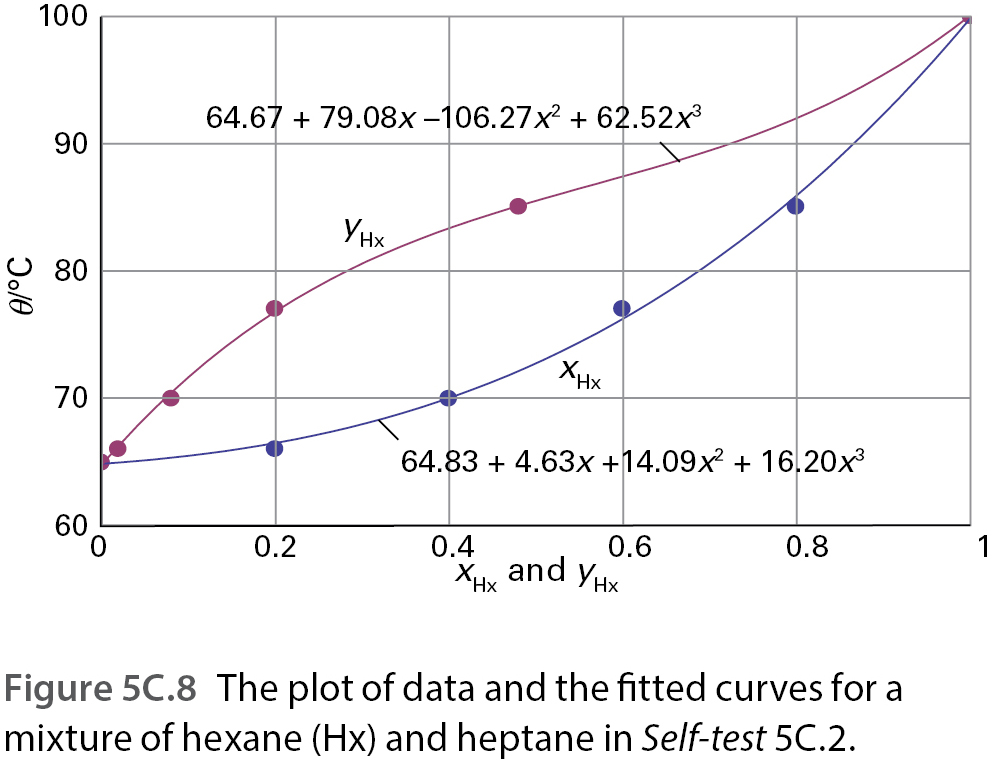
\includegraphics[width=0.6\linewidth]{Mixture_Curve}

\vspace{25em}\noindent
Below are the composition curves for a certain azeotrope. Suppose you have a sample of this mixture with composition $Z_A = a$ (the dashed line marked $a$). In the limit of a many-stage distillation carried out until compositions are stable, what will be the compositions of the liquid and vapor phases?

\noindent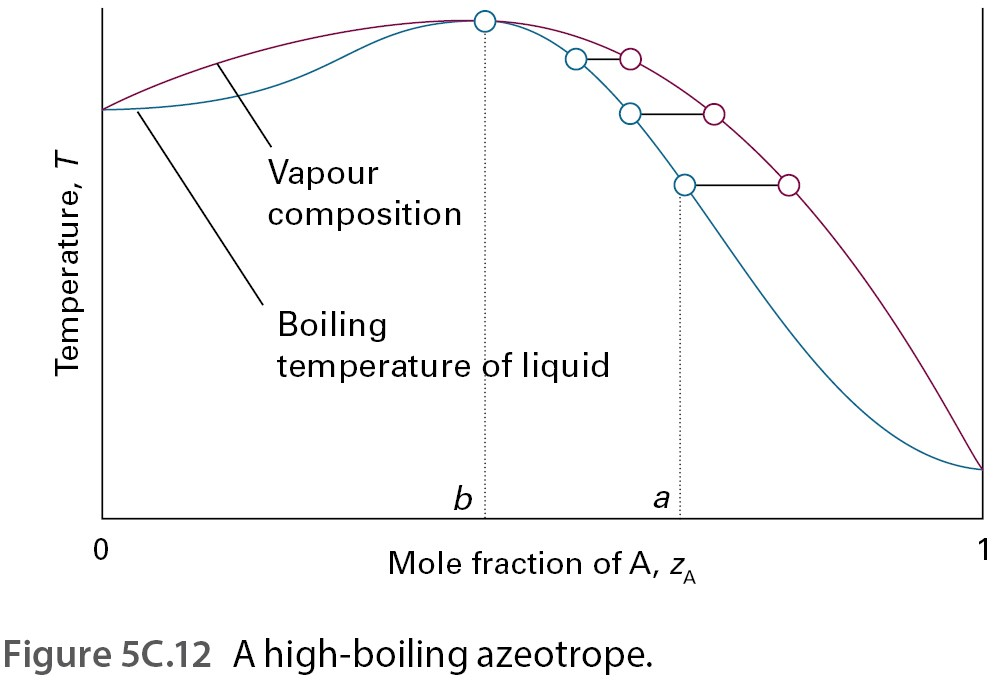
\includegraphics[width=0.6\linewidth]{Azeotrope}



\vspace{2em}\noindent
Below are the composition curves for a mixture near its freezing point. The eutectic composition ($e_2$ in the figure) is at $\chi_B = 0.42$. Suppose you have a liquid with $3.0~moles$ of $B$ and $1.0~mole$ of $A$. This mixture has $\chi_B=0.75$ ($a$ in the figure), and is cooled slowly until it just reaches the eutectic freezing point. Find the following at this point: $\circled{1}$ The compositions of the solid and liquid phases, and $\circled{2}$ the number of moles in the solid phase.

\noindent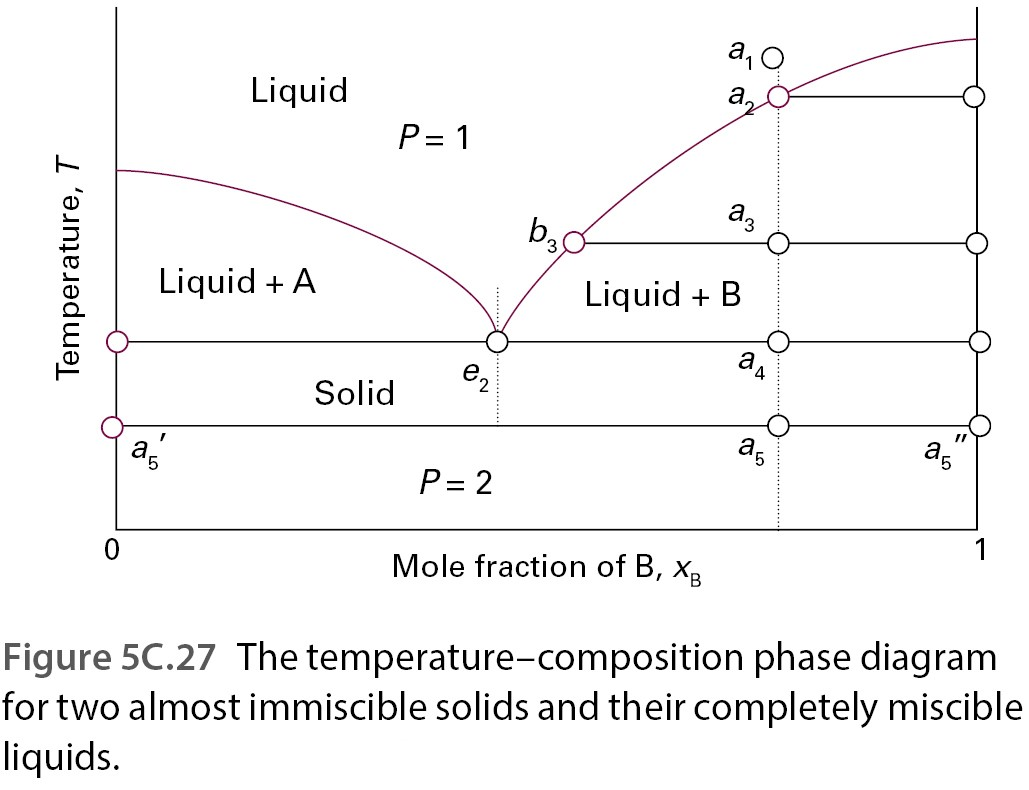
\includegraphics[width=0.6\linewidth]{Eutectic}

\vspace{2em}\noindent
\begin{minipage}{0.55\textwidth}
	\noindent At right is a diagram for two marginally miscible liquids. Consider a mixture with a temperature and composition indicated by point $b_3$.

	\noindent  $\circ$ Give the number of phases, the composition of each phase, and the approximate ratio $\frac{n_i}{n_{total}}$ for each phase
		
	\vspace{9em}
	~
	
	

\end{minipage} ~~
\begin{minipage}{0.55\textwidth}
	\noindent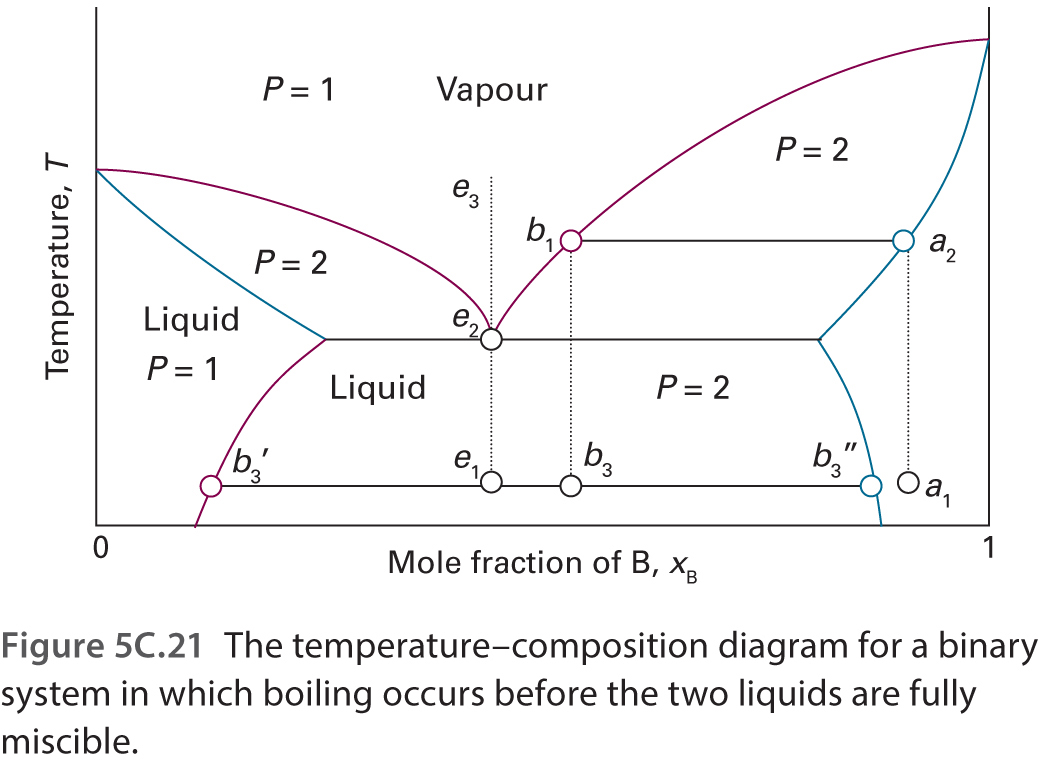
\includegraphics[width=\linewidth]{Bunny_Ears}
\end{minipage}
\noindent This mixture is then heated until it reaches the minimum boiling point marked by the azeotrope point $e2$. Note that this temperature is marked by a black line on the diagram. 

	\noindent $\circ$ Give the number of phases, the composition of each phase, and the approximate ratio $\frac{n_i}{n_{total}}$ for each phase at this temperature
	
\vspace{11em}\hspace{-4em}\noindent
\begin{minipage}{0.55\textwidth}
	\noindent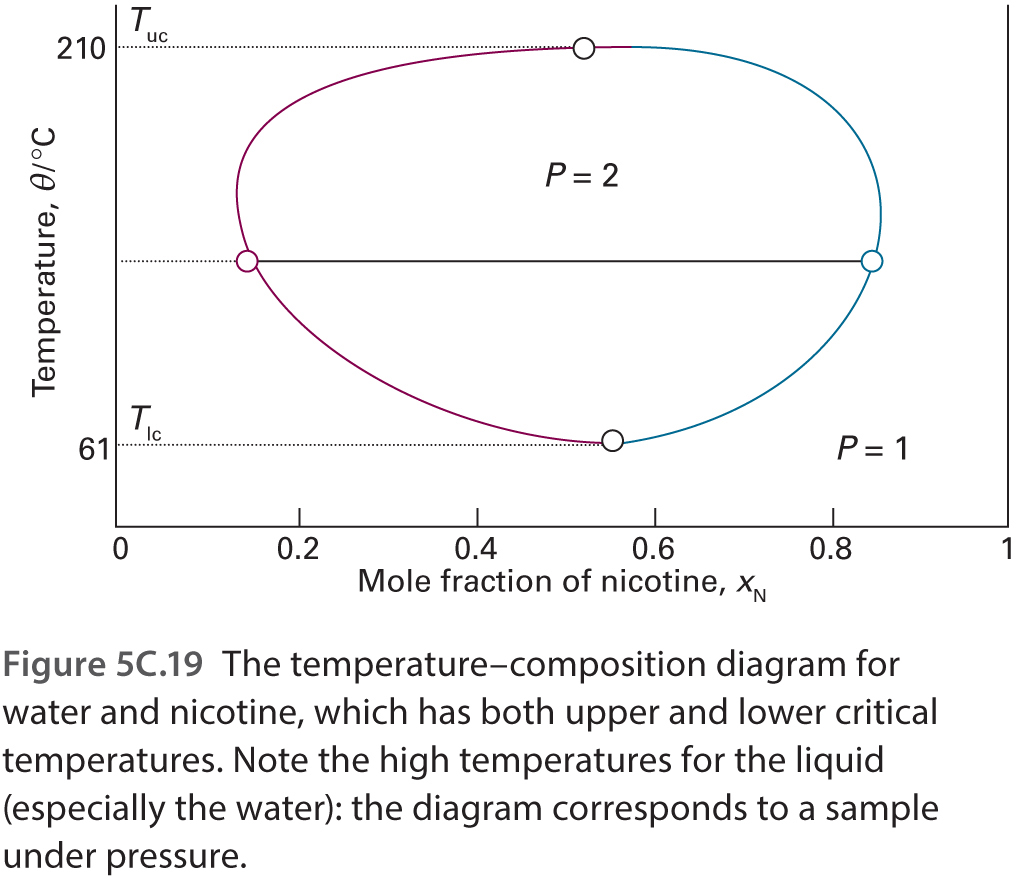
\includegraphics[width=\linewidth]{Nicotine}
\end{minipage} ~~
\begin{minipage}{0.55\textwidth}
	\noindent At left is a phase diagram for a mixture of nicotine and water
	
	\noindent $\circ$ You have a mixture with $\chi_N = 0.30$ at room temperature. As you heat the mixture, at some point it suddenly splits into two phases. At what temperature (approximately) does this split occur?
	
	\vspace{1.5em}
	\noindent As you heat the mixture, you find that one phase is much more concentrated in nicotine and you decide to use this phenomenon to purify your nicotine mixture. 
	
	\noindent $\circ$ What is the highest concentration of nicotine that you can hope to achieve?
	
	\vspace{1.5em}
	\noindent $\circ$ What fraction of the mixture will be in this concentrated phase?
\end{minipage}
	
\newpage
\pagestyle{empty}
\addtocounter{page}{-1}
\section*{\emph{{\fontspec{Malgun Gothic}귀천} (Back to Heaven)}}
\paragraph{By {\fontspec{Malgun Gothic}천상병} (Cheon Sang-byeong)}~

{\fontspec{Malgun Gothic}
	\begin{verse}
		나 하늘로 돌아가리라\\
		새벽빛 와 닿으면 스러지는\\
		이슬 더불어 손에 손을 잡고,
		
		나 하늘로 돌아가리라.\\
		노을빛 함께 단둘이서\\
		기슭에서 놀다가 구름 손짓하며는,
		
		나 하늘로 돌아가리라.\\
		아름다운 이 세상 소풍 끝내는 날,\\
		가서, 아름다웠더라고 말하리라...
	\end{verse}
}

\vspace{2em}
\begin{verse}
	I'll go back to heaven again\\
	hand in hand with the dew\\
	that melts at the touch of the dawning day,
	
	I'll go back to heaven again.\\
	After playing on the slopes with the dusk,\\
	when the clouds beckon, 
	
	I'll go back to heaven again.\\
	On the last day of my outing to this beautiful world,\\
	I'll go back and say: it was beautiful...
\end{verse}
\end{document}
